%%%%%%%%%%%%%%%%%%%%%%%%%%%%%%%%%%%%%%%%%
% Beamer Presentation
% LaTeX Template
% Version 1.0 (10/11/12)
%
% This template has been downloaded from:
% http://www.LaTeXTemplates.com
%
% License:
% CC BY-NC-SA 3.0 (http://creativecommons.org/licenses/by-nc-sa/3.0/)
%
%%%%%%%%%%%%%%%%%%%%%%%%%%%%%%%%%%%%%%%%%

%-------------------------------------------------------------------------------
%	PACKAGES AND THEMES
%---------------------------------------------------------------------------------

\documentclass{beamer}

\mode<presentation> {

% The Beamer class comes with a number of default slide themes
% which change the colors and layouts of slides. Below this is a list
% of all the themes, uncomment each in turn to see what they look like.

%\usetheme{default}
%\usetheme{AnnArbor}
%\usetheme{Antibes}
%\usetheme{Bergen}
%\usetheme{Berkeley}
%\usetheme{Berlin}
%\usetheme{Boadilla}
%\usetheme{CambridgeUS}
\usetheme{Copenhagen} %bom
%\usetheme{Darmstadt}
%\usetheme{Dresden}
%\usetheme{Frankfurt}
%\usetheme{Goettingen}
%\usetheme{Hannover}
%\usetheme{Ilmenau}
%\usetheme{JuanLesPins}
%\usetheme{Luebeck}
%\usetheme{Madrid}
%\usetheme{Malmoe}
%\usetheme{Marburg} %bom
%\usetheme{Montpellier}
%\usetheme{PaloAlto}
%\usetheme{Pittsburgh}
%\usetheme{Rochester}
%\usetheme{Singapore}
%\usetheme{Szeged}
%\usetheme{Warsaw}

}
\usepackage[brazil, english]{babel}   
\usepackage[utf8]{inputenc}  
\usepackage{graphicx} % Allows including images
\usepackage{booktabs} % Allows the use of \toprule, \midrule and \bottomrule in tables
\usepackage{ragged2e} %justify
\usepackage{multicol}
\usepackage[brazil]{babel}
\usepackage{booktabs}
\usepackage{scalefnt}
\usepackage{scalefnt}
\usepackage{amsmath}
\usepackage{graphicx}
\usepackage{scalefnt}
\usepackage{url}
\usepackage{natbib}
\ifpdf%
\usepackage{epstopdf}%
\else%
\fi
\usepackage{multirow}
\usepackage[utf8]{inputenc} 

%----------------------------------------------------------------------------------------
%	TITLE PAGE
%----------------------------------------------------------------------------------------

\title{\textbf{Título}} 
\author{Autores (Primeiro e Segundo Nome)} \\\\\\ \institute[Universidade (Sigla)] 
{
\\
\textb{Institute of Mathematical and Computer Sciences, University of São Paulo \\}\\\\\\\

\begin{minipage}[b]{0.50\linewidth}
\centering

\includegraphics[width=5.5cm]{figuras/deep-learning-book.jpg}
\end{minipage}
\medskip
}


\begin{document}
\begin{frame}
\titlepage % Print the title page as the first slide
\end{frame}

\begin{frame}
\frametitle{Summary}
\begin{enumerate}
    \item Abstract
    \item Research Gap and Contributions
    \item Research Methodology
    \item Main Concepts
    \item Data Overview
    \item Experiments
    \item Critical Paper Analysis (positive and negative points)
    \item Conclusions
\end{enumerate}
\end{frame}



%------------------------------------------------------
\begin{frame}
\frametitle{Abstract}
%------------------------------------------------------

\end{frame}


%------------------------------------------------------
\begin{frame}
\frametitle{Research Gap and Contributions}
%-----------------------------------------------------

\begin{enumerate}
    \item \textbf{Research gap}:
    \begin{enumerate}
        \item 1.
        \item 2.
    \end{enumerate}
    \item  \textbf{Main contributions:} 
    \begin{enumerate}
        \item 1
        \item 2
        \end{enumerate}
\end{enumerate}
\end{frame}

%-----------------------------------------------------
\begin{frame}
\frametitle{Research Methodology}
%-----------------------------------------------------
 \begin{figure}[!htb]
\centering  
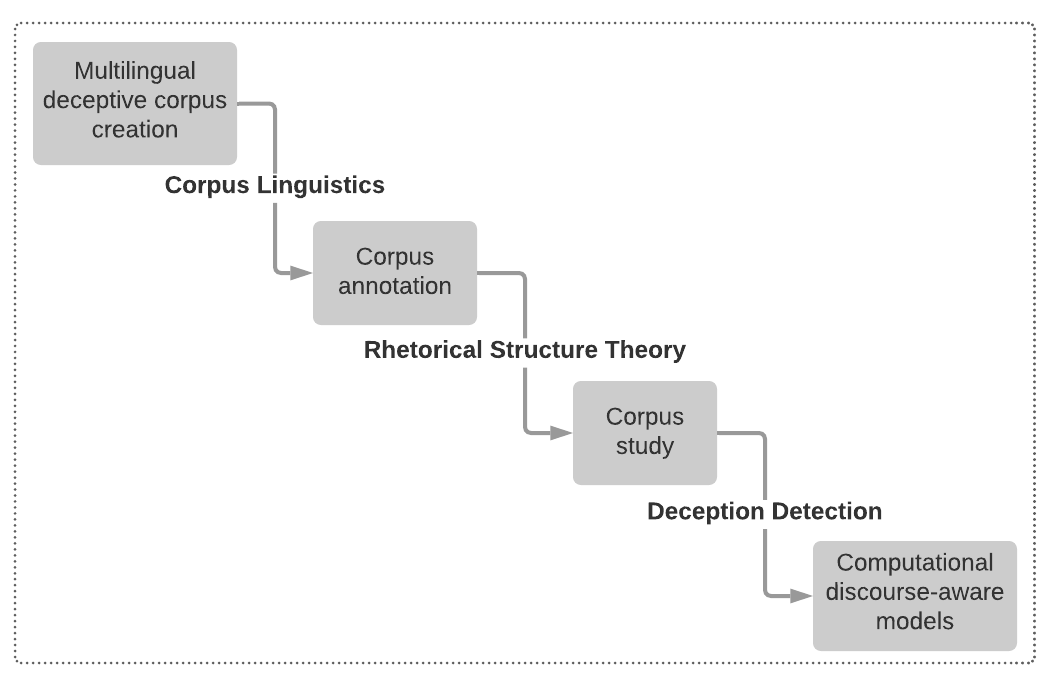
\includegraphics[width=0.85\textwidth]{figuras/methodology.png}
\caption{Methodology.}
\end{figure}
\end{frame}


%-----------------------------------------------------
\begin{frame}
\frametitle{Research Methodology}
%-----------------------------------------------------
 \begin{figure}[!htb]
\centering  
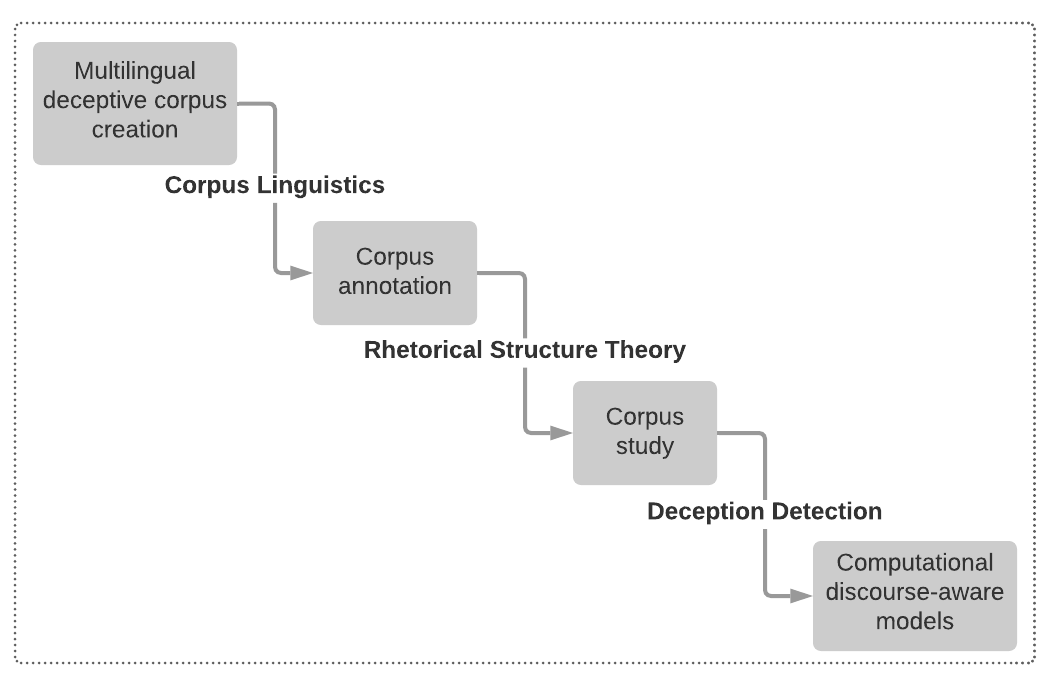
\includegraphics[width=0.85\textwidth]{figuras/methodology.png}
\caption{Methodology.}
\end{figure}
\end{frame}

%---------------------------------------------------
\begin{frame}
\frametitle{Main Concepts}
%---------------------------------------------------

\end{frame}



%---------------------------------------------------
\begin{frame}
\frametitle{Main Concepts}
%---------------------------------------------------

\end{frame}

%------------------------------------------------------
\begin{frame}
\frametitle{Data Overview}
%-----------------------------------------------------


\end{frame}

%------------------------------------------------------
\begin{frame}
\frametitle{Experiments}
%-----------------------------------------------------


\end{frame}



%------------------------------------------------------
\begin{frame}
\frametitle{Experiments}
%------------------------------------------------------

\end{frame}

%------------------------------------------------------
\begin{frame}
\frametitle{Experiments}
%------------------------------------------------------

\end{frame}


%------------------------------------------------------
\begin{frame}
\frametitle{Critical Paper Analysis (positive and negative points}
%------------------------------------------------------

\end{frame}


%------------------------------------------------------
\begin{frame}
\frametitle{Critical Paper Analysis (positive and negative points)}
%------------------------------------------------------

\end{frame}


%------------------------------------------------------
\begin{frame}{Conclusions}
 
\end{frame}

%------------------------------------------------------

%------------------------------------------------------
\begin{frame}
\frametitle{References}
%------------------------------------------------------
\small
\bibliographystyle{plain}
\bibliography{bibliografia1.bib}
\end{frame}


\end{document}